%% Computers & Geosciences (Elsevier elsarticle, Harvard author-year).
%% Publishable engine only — transport (warped) kriging is patent-pending and
%% excluded from this manuscript.
\documentclass[preprint,12pt,authoryear]{elsarticle}

\usepackage{lineno,hyperref}
\usepackage{graphicx}
\usepackage{booktabs}
\usepackage{amsmath}
\usepackage{siunitx}
\graphicspath{{../figures/}}

\journal{Computers \& Geosciences}

\begin{document}

\begin{frontmatter}

\title{geostat-rs: a single-binary Rust engine for geostatistics, validated
against gstat and bridged to machine learning}

\author[a]{Francisco Parra-O.\corref{cor1}}
\ead{}
\cortext[cor1]{Corresponding author.}
\affiliation[a]{organization={},
            city={},
            country={Chile}}

\begin{abstract}
Spatially continuous predictions from point samples underpin work across the
geosciences, yet the practical toolchain is split between \texttt{gstat}
(\textsf{R} --- feature-rich but slow and tied to the \textsf{R} runtime) and
GSLIB (Fortran --- fast but archaic, with no modern bindings). We present
\textbf{geostat-rs}, a geostatistics engine written in Rust that is
single-binary, dependency-light and reproducible across platforms, with
first-class Python and WebAssembly bindings. The core is generic over spatial
dimension (2-D and 3-D from one const-generic code path) and covers
experimental and theoretical variography; the kriging family
(simple/ordinary/universal/external-drift, co-kriging, indicator and block
kriging); inverse-distance and $k$-nearest-neighbour baselines; regression
kriging; and conditional sequential Gaussian and indicator simulation with a
deterministic, platform-independent random-number generator. Every
deterministic method is cross-checked against gstat on the Meuse and Walker
Lake benchmarks at machine precision; simulation is validated distributionally.
Following \citet{li2021}, accuracy is assessed by VEcv (variance explained by
cross-validation), method comparison and hyperparameter tuning are driven by
predictive accuracy, and regression kriging accepts an externally supplied
trend --- letting a machine-learning model provide the mean while geostat-rs
kriges the residuals. We demonstrate the engine on a national mine-tailings
geochemistry dataset, predicting rare-earth grades from cheap host-mineral
proxies. The engine reads and writes OGC GeoPackage (vector points and
single-band raster) without GDAL, for native interchange with GIS tools.
\end{abstract}

\begin{keyword}
geostatistics \sep kriging \sep Rust \sep cross-validation \sep
regression kriging \sep GeoPackage
\end{keyword}

\end{frontmatter}

%\linenumbers

\section{Introduction}
\label{sec:intro}

Spatially continuous fields --- ore grades, element concentrations, soil and
environmental variables --- are increasingly required across ecology, agronomy,
geochemistry, mining and environmental science, yet are rarely measured
exhaustively: they must be predicted from sparse point samples
\citep{li2021,goovaerts1997}. Geostatistics supplies the established machinery
for this --- variography to characterise spatial dependence, kriging to predict
with quantified uncertainty, and stochastic simulation to represent it --- and a
growing body of work couples it with machine learning for the trend component
\citep{hengl2018}. A practitioner therefore needs a single tool that spans this
whole workflow, validates against an accepted reference, and deploys without a
heavy runtime.

Two implementations anchor the field. \texttt{gstat} \citep{pebesma2004} is
comprehensive and the de-facto reference, but is bound to the \textsf{R}
runtime, single-threaded in its hot paths, and offers no single-binary or
in-browser deployment; GSLIB \citep{deutsch1998} is fast, canonical Fortran but
arcane and without modern packaging, bindings or a Python/WebAssembly interface.
The Python geostatistics ecosystem --- for example GSTools \citep{mueller2022}
and SciKit-GStat \citep{maelicke2022} --- is convenient and scriptable but
pure-Python in performance and likewise without a single-binary or client-side
target. No engine combines dependency-light single-binary deployment,
cross-platform reproducibility, a unified 2-D/3-D core, Python and WebAssembly
bindings, and numerical fidelity to gstat.

We present geostat-rs to fill that gap. Its design goals are: (i) a single
binary with no heavy runtime or GDAL chain; (ii) reproducible results across
platforms via a deterministic random-number generator; (iii) one code path for
2-D and 3-D; (iv) Python and WebAssembly bindings; (v) numerical parity with
gstat; and (vi) a predictive-accuracy-first evaluation methodology with a bridge
to machine learning, following \citet{li2021}. Our contributions are the engine
itself, its validation against gstat at machine precision, predictive-accuracy
tooling (VEcv-based comparison and tuning), an ML+geostatistics hybrid through
regression kriging, GeoPackage input/output, and a real rare-earth application.

\section{Design and implementation}
\label{sec:design}

geostat-rs is written in Rust (edition 2024) as a Cargo workspace:
\texttt{geostat-core} (the library, with no I/O and only light dependencies),
\texttt{geostat-cli} (a command-line tool), \texttt{geostat-python} (a PyO3
module, abi3 $\geq$ 3.9) and \texttt{geostat-wasm} (WebAssembly with a browser
demo). The core is generic over the spatial dimension through a const-generic
\texttt{PointSet<const D>}, so variography, kriging, cross-validation and
simulation run unchanged in 2-D and 3-D. Moving neighbourhoods use a $k$-d tree;
sequential simulation uses an incremental bucket grid. A deterministic
random-number generator (xoshiro256++) makes simulation reproducible:
the same seed yields identical realizations on any platform. Native parallelism
(rayon) is behind a feature flag that is disabled for the wasm32 target. The
Python module reproduces the CLI bit-for-bit, and the WebAssembly build runs
the same engine in the browser with no server (Figure~\ref{fig:wasm}).

\begin{figure}[t]
\centering
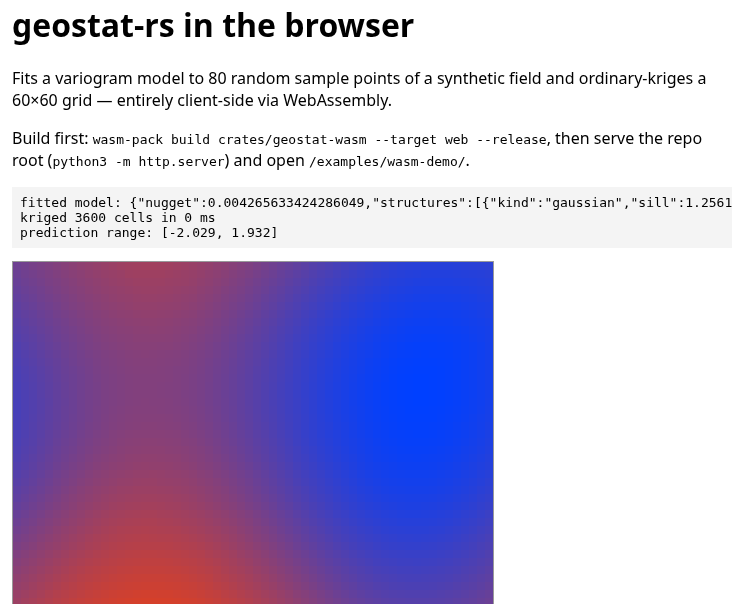
\includegraphics[width=0.7\linewidth]{fig_wasm.png}
\caption{The WebAssembly build running entirely client-side in a browser: it
fits a variogram and ordinary-kriges a $60\times60$ grid of a synthetic field,
rendering the prediction surface on a canvas.}
\label{fig:wasm}
\end{figure}

\section{Methods}
\label{sec:methods}

\textbf{Variography.} Experimental variograms (omnidirectional, directional with
azimuth and a 3-D dip cone) and cross-variograms; theoretical models (spherical,
exponential, Gaussian, Mat\'ern $\nu=3/2,5/2$), nested with a nugget and with
geometric anisotropy; weighted-least-squares fitting with gstat's default
$N_j/h_j^2$ weights via Nelder--Mead, with automatic best-family selection.

\textbf{Kriging.} Simple, ordinary, universal (polynomial drift) and
external-drift kriging; ordinary co-kriging (collocated and heterotopic) under a
linear model of coregionalization; block kriging and block co-kriging; indicator
kriging (local ccdf, E-type estimate, conditional variance); and lognormal
kriging.

\textbf{Mathematical interpolators.} Inverse-distance weighting and
$k$-nearest-neighbour averaging ($k=1$ is nearest-neighbour / Voronoi) as
assumption-light baselines for fair comparison \citep{li2021}.

\textbf{Regression kriging.} A trend is fitted in a separate first step ---
either the built-in ordinary-least-squares trend or any external model --- and
the residuals are kriged and added back. Decoupling the trend lets it come from
any regressor, including machine learning \citep{hengl2018,li2021}.

\textbf{Simulation.} Conditional sequential Gaussian simulation (normal-score
transform) and sequential indicator simulation with order-relation corrections,
both with the deterministic generator.

\textbf{Predictive-accuracy tooling.} Following \citet{li2016}, leave-one-out
cross-validation reports VEcv ($=100\,[1-\sum(y-\hat y)^2/\sum(y-\bar y)^2]$, a
scale- and variance-independent cross-validated $R^2$) and the Legates--McCabe
$E_1$, alongside scale-free relative measures. A harness ranks methods by VEcv
on the same data, and hyperparameters (IDW power, $k$-NN $k$, kriging
neighbourhood size) are tuned by maximizing VEcv rather than by a model fit.

\textbf{Input/output.} CSV; OGC GeoPackage point layers (read and write) and
single-band 2D-gridded-coverage raster (read and write, integer datatype),
implemented in pure Rust via bundled SQLite and a PNG codec, i.e.\ without a
GDAL dependency; a read raster can be sampled at point locations to attach a
covariate (e.g.\ a DEM) for external-drift or regression kriging.

\section{Validation against gstat}
\label{sec:validation}

Every deterministic method is cross-checked against gstat on the Meuse and
Walker Lake benchmarks. Table~\ref{tab:parity} lists headline parities; the full
tables are in the repository. Conventions are aligned with gstat where they
matter: the semivariance estimator, right-closed lag bins, $N_j/h_j^2$ fit
weights, azimuth measured clockwise from north and nugget-free within-block
covariance. Figure~\ref{fig:parity} shows geostat-rs against gstat on the Meuse
grid for ordinary kriging and IDW: predictions lie on the identity line to
machine precision. Simulation is validated distributionally --- a
1000-realization sequential Gaussian ensemble reproduces the theoretical
simple-kriging mean and standard-deviation fields and the pooled quantiles,
while running about $7\times$ faster than gstat.

\begin{table}[t]
\centering
\caption{Maximum difference between geostat-rs and gstat (Meuse / Walker Lake).}
\label{tab:parity}
\begin{tabular}{@{}lll@{}}
\toprule
Method & Check & Max difference \\
\midrule
Experimental variogram & $\gamma$ (relative), 15 lags & \num{1.6e-15} \\
Ordinary kriging & meuse.grid, 3103 cells & \num{1.5e-12} \\
LOO cross-validation & 155 points & \num{9.7e-13} \\
KED / anisotropy / co-kriging & predictions & $\leq$\,\num{1.5e-12} \\
Block / 3-D / heterotopic co-kriging & predictions & $\leq$\,\num{4e-14} \\
Indicator kriging (in range) & $F(\text{cutoff})$ & \num{7.4e-10} \\
Lognormal (simple) kriging & vs gstat SK + analytic & \num{1.2e-9} \\
Inverse-distance weighting & power 2, global & \num{1.9e-14} \\
\bottomrule
\end{tabular}
\end{table}

\begin{figure}[t]
\centering
\includegraphics[width=\linewidth]{fig_parity.pdf}
\caption{geostat-rs versus gstat predictions on the Meuse grid for ordinary
kriging and inverse-distance weighting; points lie on the identity line (dashed)
to machine precision.}
\label{fig:parity}
\end{figure}

\section{Performance}
\label{sec:performance}

Table~\ref{tab:bench} times ordinary kriging on regular grids of increasing
size and leave-one-out cross-validation, conditioning on the 155 Meuse points
with a 32-point moving neighbourhood and the same fitted model. Only the
operation is timed (data preloaded, best of three runs); geostat-rs is timed
through its Python binding (a thin wrapper over the Rust compute) against
gstat~2.1.4. Single-threaded, geostat-rs is already faster than gstat at grid
kriging ($1.2$--$2\times$); with its parallel moving-neighbourhood predictor on
16 cores it is $6$--$12\times$ faster. Leave-one-out cross-validation is far
faster still, as gstat's \texttt{krige.cv} carries per-fold R-level overhead
that the parallel Rust implementation avoids. For a global neighbourhood the
kriging-system matrix is identical for every target, so geostat-rs factorizes it
once (LU) and only back-substitutes per target, an order-of-magnitude saving on
large grids.

\begin{table}[t]
\centering
\caption{Wall-clock time (ms, best of 3) for ordinary kriging and
leave-one-out cross-validation. Hardware: 12th-gen Intel Core i7-1270P
(16 logical cores); gstat 2.1.4 single-threaded.}
\label{tab:bench}
\begin{tabular}{@{}lrrrr@{}}
\toprule
Task & gstat & \shortstack[r]{geostat-rs\\(1 core)} &
\shortstack[r]{geostat-rs\\(16 cores)} & speedup \\
\midrule
OK grid, 2\,500 cells   & 184  & 89   & 15  & $12\times$ \\
OK grid, 10\,000 cells  & 570  & 472  & 60  & $10\times$ \\
OK grid, 40\,000 cells  & 2173 & 1595 & 341 & $6\times$ \\
LOO cross-validation (155 pts) & 1368 & 8.9 & 5.2 & $263\times$ \\
\bottomrule
\end{tabular}
\end{table}

\section{Predictive accuracy, comparison and tuning}
\label{sec:accuracy}

On Meuse log-zinc, leave-one-out VEcv ranks ordinary kriging
($\approx 71$) above IDW and $k$-NN ($\approx 54$) and nearest-neighbour
($\approx 38$) (Figure~\ref{fig:compare}); no method dominates universally, so
the comparison is by measured predictive accuracy rather than assumption.
Hyperparameters are tuned the same way: Figure~\ref{fig:idwtune} shows IDW power
selected by VEcv, with an optimum near power~3.5 on this dataset.

\begin{figure}[t]
\centering
\includegraphics[width=0.85\linewidth]{fig_compare.pdf}
\caption{Leave-one-out VEcv by method on Meuse log-zinc.}
\label{fig:compare}
\end{figure}

\begin{figure}[t]
\centering
\includegraphics[width=0.85\linewidth]{fig_idw_tune.pdf}
\caption{IDW power tuned by predictive accuracy (leave-one-out VEcv) on Meuse
log-zinc.}
\label{fig:idwtune}
\end{figure}

\section{Application: rare-earth grade prediction with an ML hybrid}
\label{sec:application}

We predict rare-earth grades on $\sim$1100 mine-tailings deposits, drawn from the
public geochemical registry of tailings deposits in Chile
\citep{sernageomin2023}, from non-rare-earth
host-mineral proxies (P$_2$O$_5$, Th for phosphates/monazite; TiO$_2$,
Fe$_2$O$_3$, Zr for Ti--Fe oxides and zircon), deliberately excluding
neighbouring rare-earth elements, which are co-measured and would constitute
leakage. Hold-out VEcv (Table~\ref{tab:ree}, Figure~\ref{fig:ree}) shows that
covariate value tracks the geochemistry: light rare earths (Ce, Nd, Dy) follow
the phosphate proxies, the heavy proxy set predicts Y, and La carries no signal
in any predictor (all methods negative --- the engine does not manufacture
signal). The random-forest-trend plus residual-kriging hybrid is best or tied
wherever signal exists. The random-forest trend is supplied by a companion Rust
machine-learning engine and the residual kriging by geostat-rs, giving an
RFOK-style hybrid \citep{li2021} with no \textsf{R} or scikit-learn dependency.

\begin{table}[t]
\centering
\caption{Hold-out VEcv (\%) by rare-earth element and method (Coquimbo
tailings; host-mineral proxies). Skew of the grade is shown for context.}
\label{tab:ree}
\begin{tabular}{@{}lrrrrr@{}}
\toprule
Element & skew & OK & RK (OLS) & RF & RF+res.\ krige \\
\midrule
La & 10.3 & $-10.5$ & $-5.6$ & $-12.4$ & $-7.5$ \\
Ce & 5.9 & 13.3 & 39.9 & 49.9 & 51.0 \\
Nd & 6.2 & 23.4 & 59.8 & 68.9 & 70.9 \\
Dy & 3.0 & 10.1 & 35.2 & 46.1 & 52.1 \\
Y  & 0.5 & 28.9 & 64.8 & 62.3 & 66.4 \\
\bottomrule
\end{tabular}
\end{table}

\begin{figure}[t]
\centering
\includegraphics[width=\linewidth]{fig_multielement.pdf}
\caption{Rare-earth grade prediction by element and method (hold-out VEcv).
Covariate value tracks the host-mineral geochemistry; the ML-trend plus
residual-kriging hybrid is best where signal exists.}
\label{fig:ree}
\end{figure}

\section{Discussion and limitations}
\label{sec:discussion}

geostat-rs shows that a single Rust core can deliver the classical
geostatistical workflow --- variography, the kriging family and stochastic
simulation --- at numerical parity with gstat while adding cross-platform
reproducibility, native parallelism, and Python and in-browser deployment from
one code base. Pairing that core with a predictive-accuracy-first evaluation
layer (VEcv-based comparison and tuning) and bring-your-own-trend regression
kriging connects classical geostatistics to the machine-learning workflow
without leaving the engine or adding an \textsf{R} or scikit-learn dependency.

Several limitations bound the present scope. Kriging systems are solved by dense
LU factorization: this is robust for the moving-neighbourhood regime that
dominates practice, and for a global neighbourhood the single-factorization
reuse keeps large grids tractable, but it does not target the very large dense
or sparse systems for which approximate or covariance-tapering solvers would be
required. Computation is CPU-only and single-machine --- there is no GPU path
and no out-of-core or distributed mode --- so problem size is bounded by memory.
GeoPackage support reads and writes vector points and integer raster coverages,
but the float (TIFF-tile) coverage datatype and additional formats remain to be
added.
Validation and benchmarking here target the classical datasets (Meuse, Walker
Lake) and a single regional application; a broader empirical study across data
types and scales is left for future work, and the predictive-accuracy
comparison is deliberately confined to the methods in the engine rather than
surveying the wider machine-learning literature.

Future directions include GPU and out-of-core execution for larger grids,
additional input/output formats and full GeoPackage raster support for tighter
GIS interchange, and broader application studies. The deterministic,
dependency-light design is intended to make geostat-rs usable both as a
standalone tool and as an embeddable component of larger Rust geocomputing
pipelines, with results that remain reproducible across the platforms on which
it runs.

\section{Software availability and reproducibility}
\label{sec:availability}

geostat-rs is released under MIT or Apache-2.0, with crates for the core, CLI,
Python and WebAssembly. All validations are reproduced by the R reference
scripts and Python comparison scripts in the repository, and all figures by the
provided data-generation and plotting scripts. Results are deterministic and
platform-independent. The Meuse and Walker Lake benchmark datasets are
distributed with \textsf{gstat}; the rare-earth application uses the public
geochemical registry of tailings deposits in Chile \citep{sernageomin2023},
openly available from the national geology and mining service.

\section*{Acknowledgements}
%% TODO

%% Bibliography
\bibliographystyle{elsarticle-harv}
\bibliography{refs}

\end{document}
